\subsection{Sparx Systems Enterprise Architect}
Sparx Systems \entArch~is another tool that provides modeling of UML diagrams.
It supports mind map diagrams and project management, to provide full traceability from requirements specification to deployment end implementation.
This tool also provides some metrics evaluation to compute the complexity of a project based on Use Case diagrams. 

To perform this evaluation, the user needs to provide a level of implementation complexity for each interaction with authors. 
This task can be done when defining the Use Case descriptions or when performing the metrics evaluation.

To evaluate the metrics, \entArch~has a wizard which enables other options for the complexity analysis.
These options manipulate the \emph{Technical} and the \emph{Environment} complexities and are used to adapt the evaluation and perform a better result on estimation.

This system enables filtering the Use Cases used in evaluation, both on manual selection or regular expressions over use case name.
%Also can be filtered the Use Cases used in evaluation. 
%To filter can be used manual selection or regular expressions over use case name.
This kind of filtering enables the project to be distributed and evaluated individually.

\subsubsection{Results}
For use this tool in metrics calculation, the user have the possibility to do some tweaking over use case complexity (on their description) to get more precise results.
This complexity admits simple values like low, medium or high.

\entArch~offers a wizard which enables the edition of factors related to environment and technics complexity or even the hour rates, as we can see on the left side of Figure \ref{img:sparxRes}
%Some factors related to environment and technics complexity could also be edited or about hour rates in the wizard shown on the left side of Figure \ref{img:sparxRes}.
Here we can use multiple factors to evaluate this factors, like usability or portability on technical complexity.

We can also access a Use Case metrics wizard, as we can see in the right side of Figure \ref{img:sparxRes}, which illustrates the set of default values used to evaluate the effort of the task.
A set of predifined values are based on the factors edited on the previous wizard.

\begin{figure}[!htbp]
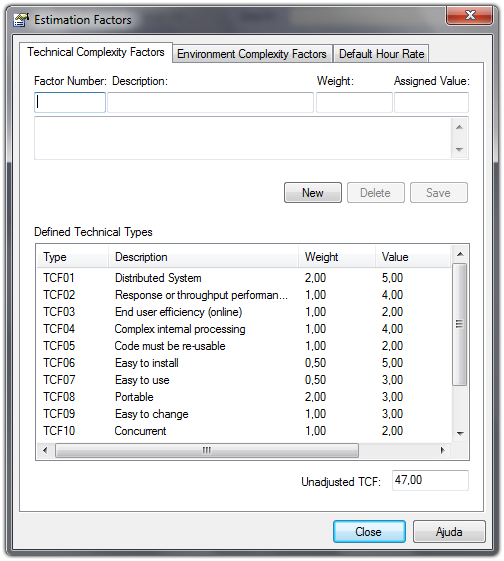
\includegraphics[scale=0.257]{images/sparxestim.png}
\hspace{0.1cm}
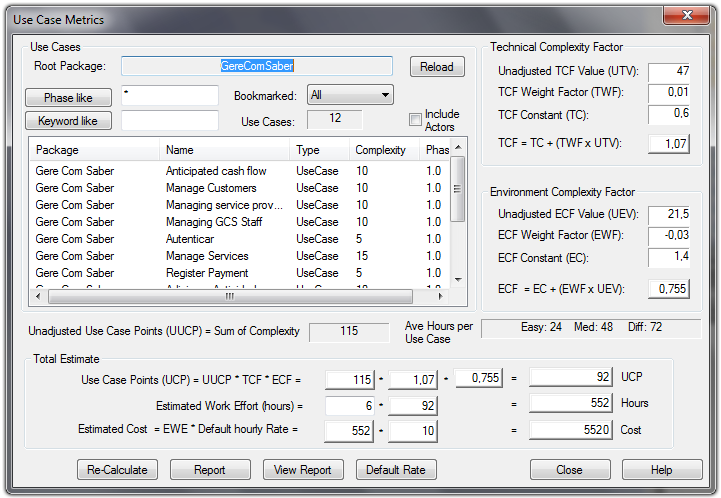
\includegraphics[scale=0.29]{images/sparx.png}
\caption{Estimation Factors and Use Case Metrics of \entArch~wizards}\label{img:sparxRes}
\end{figure}

The final result of the metrics evaluation process is an estimation of Working Hours, Use Case Points\cite{Ribu01estimatingobject-oriented} and Total Cost needed to perform the system development.

In our case-study, the project has twelve Use Cases and many of them have medium complexity. 
Thus, as we can see in the right side of Figure \ref{img:sparxRes}, the effort to complete the task is 552 working hours, that would give a final result of \EUR{5.520}. 
For obtaining this value only was changed the use cases complexity and everything else was left with default values.
